\chapter{Methods and Materials}
\label{methods}
\paragraph{Develop an online spaced repetition learning environment}
\paragraph{Visualise student usage of the learning environment}
\paragraph{Predict student responses to flash cards}

\section{Experimental Design}
\section{Participants}
\subsection{Participant Recruitment}
Participants were students of the introductory Japanese course JAPN1023. The author
introduced the project in the first week of classes and handed out registration cards
to students who chose to participate and signed a participant consent form.

\subsection{Ethical Clearance}
\label{methods_ethical}
As with any project involving humans, the details of the project must be reviewed and 
approved by the University Human Ethics Committee prior to any student participation.

An application for review was submitted in June and approved with modifications
on 25 July 2012 in time for the second week of semester.

The application included details of the methods of data collection, recruitment of participants,
and approval by a `Gatekeeper' who provides access to participants - in this case the course coordinator of JAPN1023, Dr Yuriko Nagata.

Data was to be stored anonymously and securely. In order to ensure participation was anonymous,
cards containing unique codes were to be handed out randomly to participants to allow them to
register online. Student review data was tied to a unique number in the database which could
not be traced back to individual students. Email addresses were collected from students in order
to allow them to log in and to reset their password if required, however exported review data was
stored only against a unique number in the database which could not be traced back to individual
students. Participants were also given an information sheet (See Appendix
\ref{appendix_participant_info_sheet}) and a consent form (See Appendix
\ref{appendix_participant_consent_form}) to sign and return before receiving a registration card.

\section{Online Learning Software Design}
\label{methods_softwaredesign}
\subsection{Requirements}

A number of requirements were set out for the online learning software. These are listed below along
with how these requirements are achieved.

\paragraph{Should be easily accessible to students.} Removing barriers to use will
encourage students to use the software more often. %TODO Reference

By providing access to the learning environment online via a web-based interface, students can
access the software anywhere - including from university computers without requiring installation
of any software.

\paragraph{Should be secure and anonymous.} Both for peace of mind for students, and to fulfill
ethical requirements data must be collected anonymously and securely. Students may be more
reluctant to use the software with the knowledge that their individual progress is being tracked. %TODO Ref

This is achieved by allocating each student a unique code with which the log in. Students are then
recorded in the database using a newly assigned number which is unknown to the users. Downloaded review
data should only refer to users with this number, meaning that even if the registration code is known,
a user cannot be identified from downloaded review data. Furthermore, all data should be stored on a secure
password protected server and all usage of the system via a secure connection to the server.

\paragraph{Should be easy to update and/or fix bugs.} Since the timespan is 

\paragraph{Data should be captured and stored immediately.} Since the project period is short,
users cannot be relied upon to submit their data manually in time for analysis. Therefore reviews
should be recorded immediately.

\paragraph{Only nominated students should be able to access the system}

\subsection{Tools}
This section outlines the software tools that will be used for the project and reasoning for
choosing these tools.
\paragraph{Git and Github}
(\url{http://git-scm.com/}),
(\url{http://www.github.com/})

Git is a distributed version control system (VCS) which tracks changes
to source code (often amongst multiple developers) and keeps a complete history
of changes. This is invaluable when a change in code occurs that results in a critical
bug. Versions can be compared to find the change that introduced the bug, and production
code can be reverted if need be \cite{scott_chacon_pro_2009}.

Git repositories can be hosted anywhere, however Github offers free Git repository hosting
for open source projects. It also allows
users to 'fork' public repositories to create their own version of a project. For this
reason it is useful for research projects as the project can be picked up and continued
at any time by others.

Git was selected for this project because of its portability (moving repositories
between servers is trivial). Github was chosen as it is free, encourages collaboration and is also the tool of choice for the 
Centre of Educational Innovation in Technology \cite{zornig_ceit_2012} under which this project was completed. 

\paragraph{Ruby on Rails}
(\url{http://www.rubyonrails.org/})

Ruby on Rails (aka Rails) is a popular open source framework for developing web applications\cite{bachle_ruby_2007}.
Rails was originally extracted from a commercial application (Basecamp by 37Signals) to create a generic
application framework \cite{carneiro_jr._beginning_2010} written in the Ruby language. Rails is designed for
rapid development and provides many guidelines which the developer is recommended to follow in order to speed up
development. Additionally, as an open source project Rails has gained many developers who have contributed back
to the community by sharing reusable components (known as Ruby Gems) with the community. This means many pieces of
functionality can be used in a project without rewriting, speeding up the development process. Gems used in this
project include:
\begin{description}
\item[Prawn] Provides PDF output - used for generating registration code cards
\item[CanCan] User authorisation - Allow and deny access to users based on their role (participant, administrator, teacher)
\item[Highcharts-Rails] Adds the Highcharts library to the application (See section below)
\end{description}

% TODO Complete Rails section

\paragraph{Heroku}
(\url{http://www.heroku.com/})

Heroku is a private company offering hosting for Ruby on Rails applications with automated deployment. While deploying
a Rails application on a server normally requires system administrator knowledge and a significant amount of
time to install, Heroku
allows deployment via Git and automatically installs dependencies to get an application up and running in less
than a minute.

Heroku was chosen over a private server for this project since it was necessary to be able to push updates
to the live application quickly in order to respond to bugs and to reduce time spent finding faults in the server.

% TODO Complete Heroku section

\paragraph{Backbone.JS}
(\url{http://www.backbonejs.org/})

Backbone.js is an open source Javascript framework providing a model oriented structure
for Javascript heavy web applications. Backbone.js allows data to be easily linked
to user interface components and synchronise with the server, so that any changes
to the underlying data automatically update the user interface. 
It was selected because of its integration with Ruby on Rails and because of the
author's familiarity with the library.

\paragraph{Highcharts}
(\url{http://www.highcharts.com/})

Highcharts is a commercial Javascript framework which provides graphing capabilities to web sites. Highcharts
allows free usage by non-commercial projects. Highcharts was selected for graphing usage statistics
on the website because of the features it provides in addition to recommendations on websites such as Stack Overflow \cite{stackoverflow_highcharts_2012}.
% TODO Complete Highcharts section

\paragraph{Twitter Bootstrap}
(\url{http://twitter.github.com/bootstrap})

Twitter Bootstrap is a set of default styles for websites and web applications,
provided as open-source by Twitter. Using Twitter Bootstrap rapidly speeds up theming of
a web application with default looks for navigation, buttons, text and layout.


See figure \ref{twitterbootstrap} for a comparison of default styling with and without Twitter Bootstrap
\begin{figure}[h!]
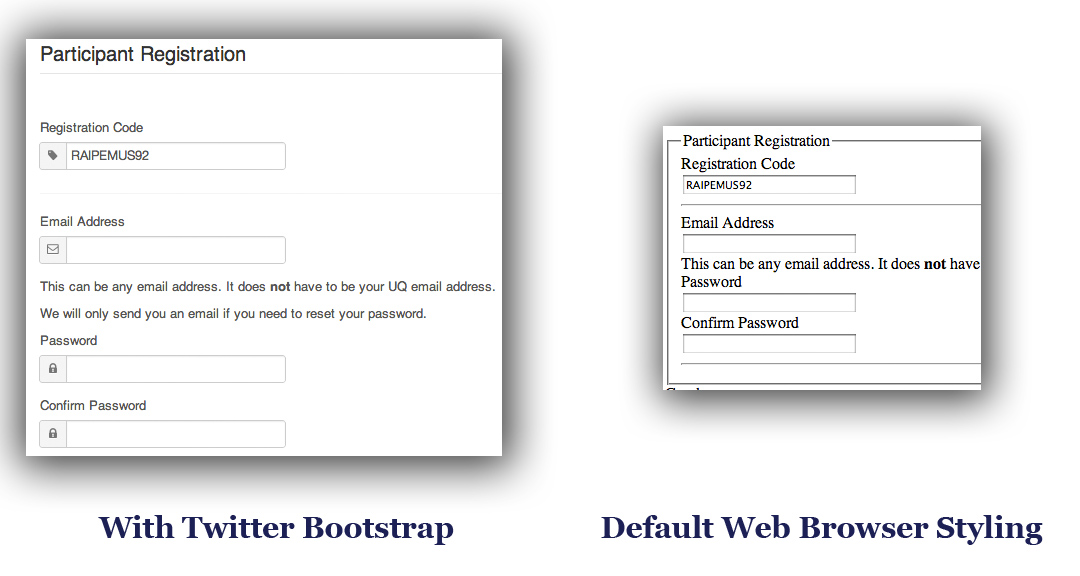
\includegraphics[width=120mm]{img/twitterbootstrap.jpg}
\caption{Comparison of a page with no styling and Twitter Bootstrap default styling}
\label{twitterbootstrap}
\end{figure}

More significantly, Twitter Bootstrap offers a `responsive' layout 
system which provides a reduced screen size (ie. smartphone) layout
 with little to no extra work on the part of the developer. This 
 means a smartphone version of the web application could be designed
  at the same time. Twitter Bootstrap was also chosen for this reason.
  
\paragraph{The R Programming Language}
R is an open source programming language designed primarily for statistical computing.
Many packages are available for R which provide functionality including various
machine learning algorithms.

R was selected since it is open source and therefore code written is possible for others to recreate
the experiment without purchasing expensive software such as MATLAB. Additionally, the libraries
available in R (such as e1071, the Support Vector Machine library) generally provide more customisability
over those available in MATLAB as standard.

\subsection{Functionality}
\subsubsection{Reviewing}
The review interface was designed with a responsive Javascript frontend in order
to reduce lag between reviews. While a student is reviewing a flash-card, the following
card is pre-loaded and displayed immediately after a response is selected.
\begin{figure}
\fbox{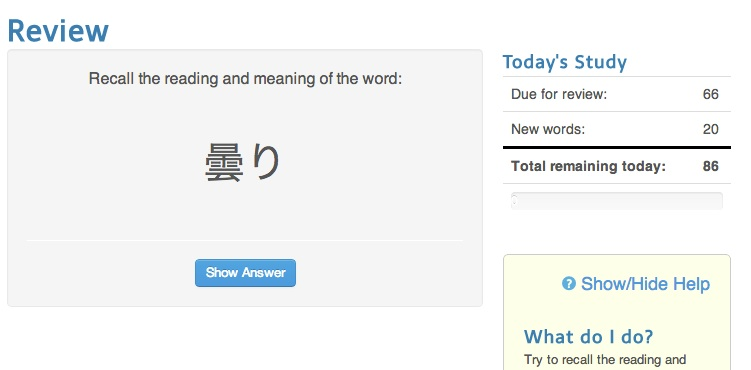
\includegraphics[width=11cm]{img/review_front.jpg}}
\caption{The `front' of a flash-card during review}
\label{fig_review_front}
\end{figure}

\begin{figure}
\fbox{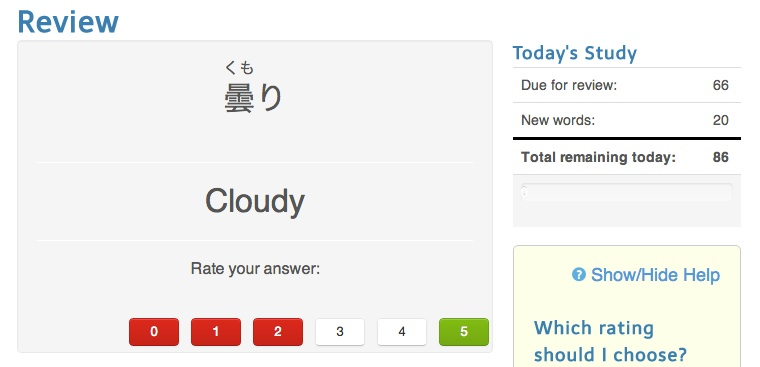
\includegraphics[width=11cm]{img/review_back.jpg}}
\caption{The `back' of a flash-card during review. Here the user is asked to rate
their response}
\label{fig_review_back}
\end{figure}

Figures \ref{fig_review_front} and \ref{fig_review_back} show the `front' and `back' of the
flash-cards respectively. The user is prompted to recall the pronounciation and English
meaning of the word on the front, then after choosing to reveal the answer can compare
their answer with that written on the back.

Finally the user rates their recall on the 0-5 scale using either the buttons on screen or
the keyboard, and the next card is then displayed.

\subsubsection{Withdrawal of Participation}
A condition of ethical approval, participants are able to withdraw
from participation from within the software at any time
using the `Withdraw Participation' function which immediately deletes all associated
information.

\subsubsection{Password Reset and Change}
Students are able to reset their password by entering their email address into a
password reset page. An email is sent containing a new random password which they
can use to log in and then change their password.
 

\subsubsection{Administration}
An secured administration section was built to facilitate the operation of system, including
features such as:
\begin{itemize}
  \item Generating registration codes
  \item Viewing error logs
  \item Downloading anonymised formatted review data
\end{itemize} 

\subsubsection{Registration Codes}
An interface for the administrator allows generation of registration codes. Registration
codes are strings of random numbers and letters which can be used to create an account.
Each code can be used only once, and is associated with a role in the system which carries
over to the account created with the code. For example, the administrator may wish to
create 50 participant codes, 5 tester codes and 1 teacher code which can then be given
to the respective users. This ensures a hard limit on the number of each type of user
that can register.

The system also provides an interface for printing sheets of registration codes on cards.
This allows the sheets to be printed onto card and cut out to be individually handed
to students. With over 100 students in the class, this feature was added to reduce the
time in writing out 100 individual cards by hand.

\begin{figure}
\fbox{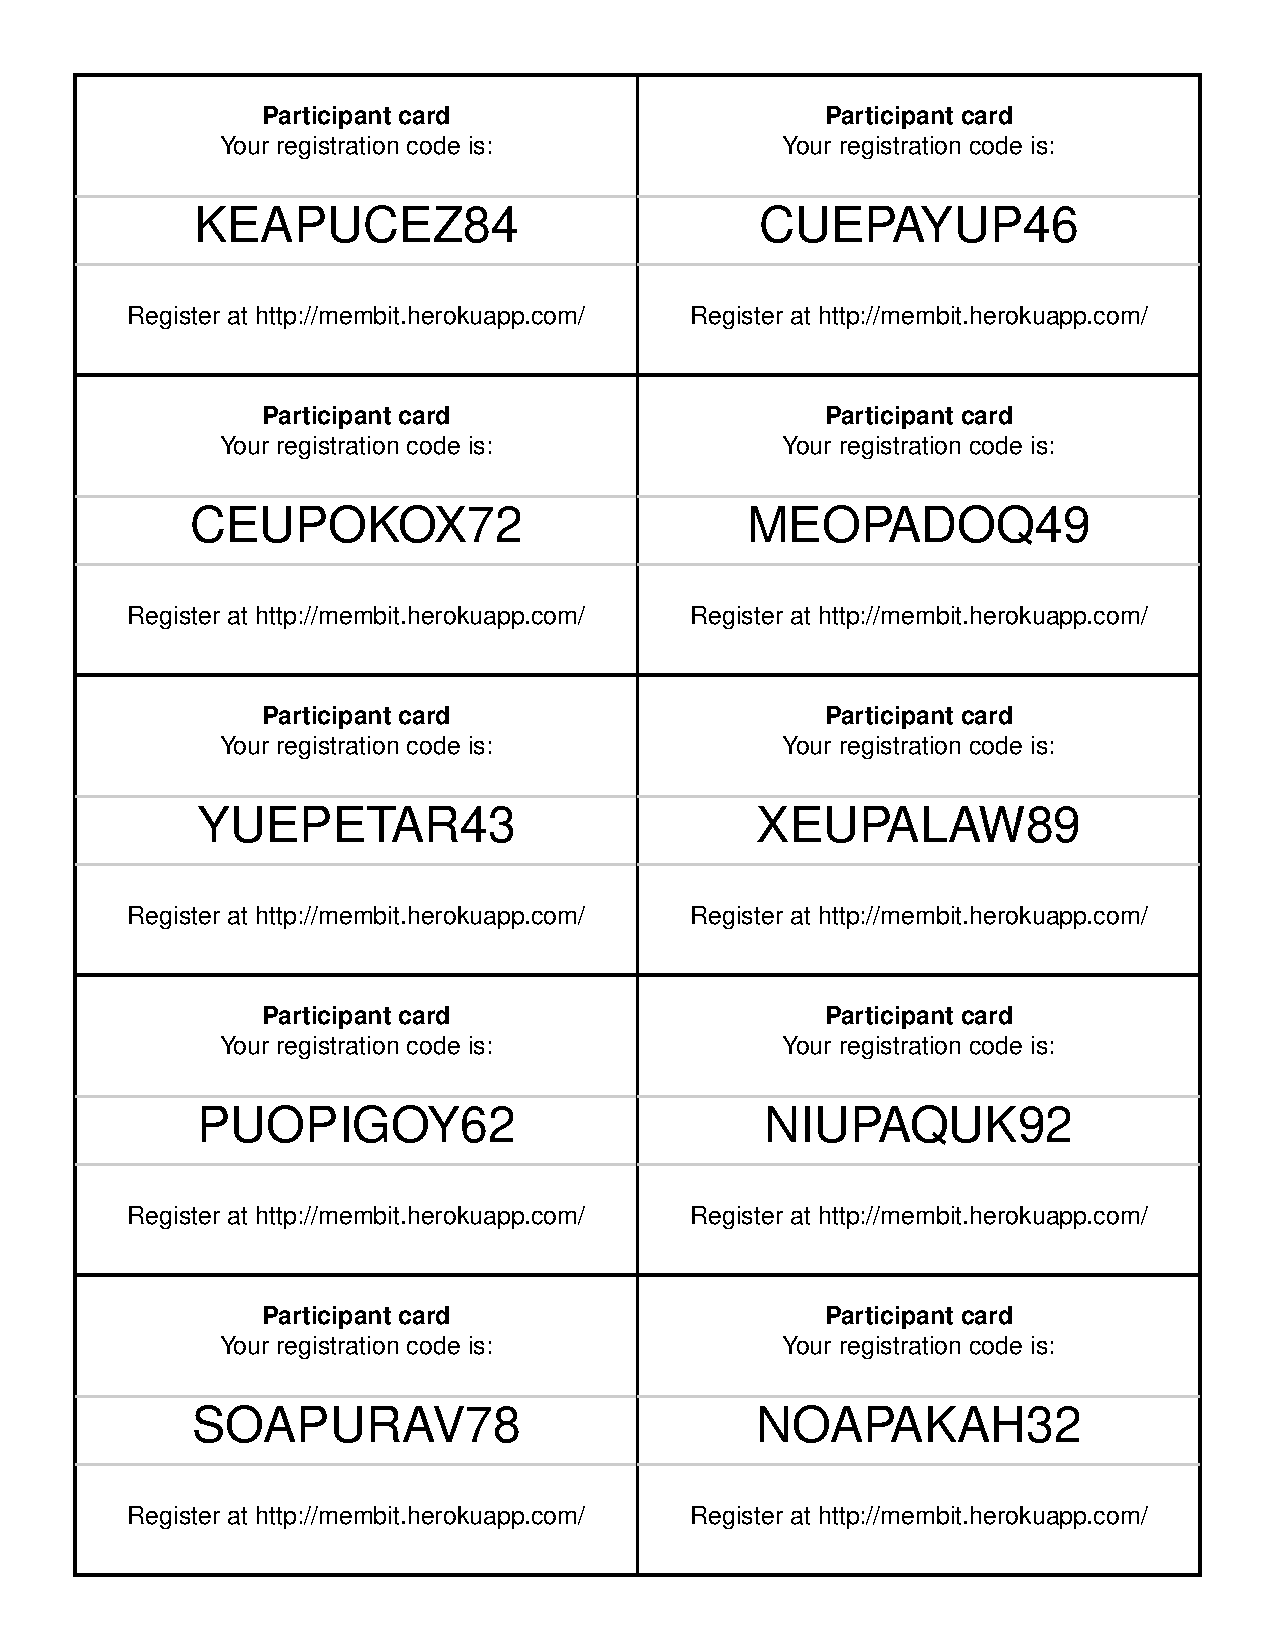
\includegraphics[page=1,width=6cm]{img/Registration_Codes.pdf}}
\caption{Sample printout of registration codes}
\label{fig_registrationcodes}
\end{figure}

\begin{figure}
\fbox{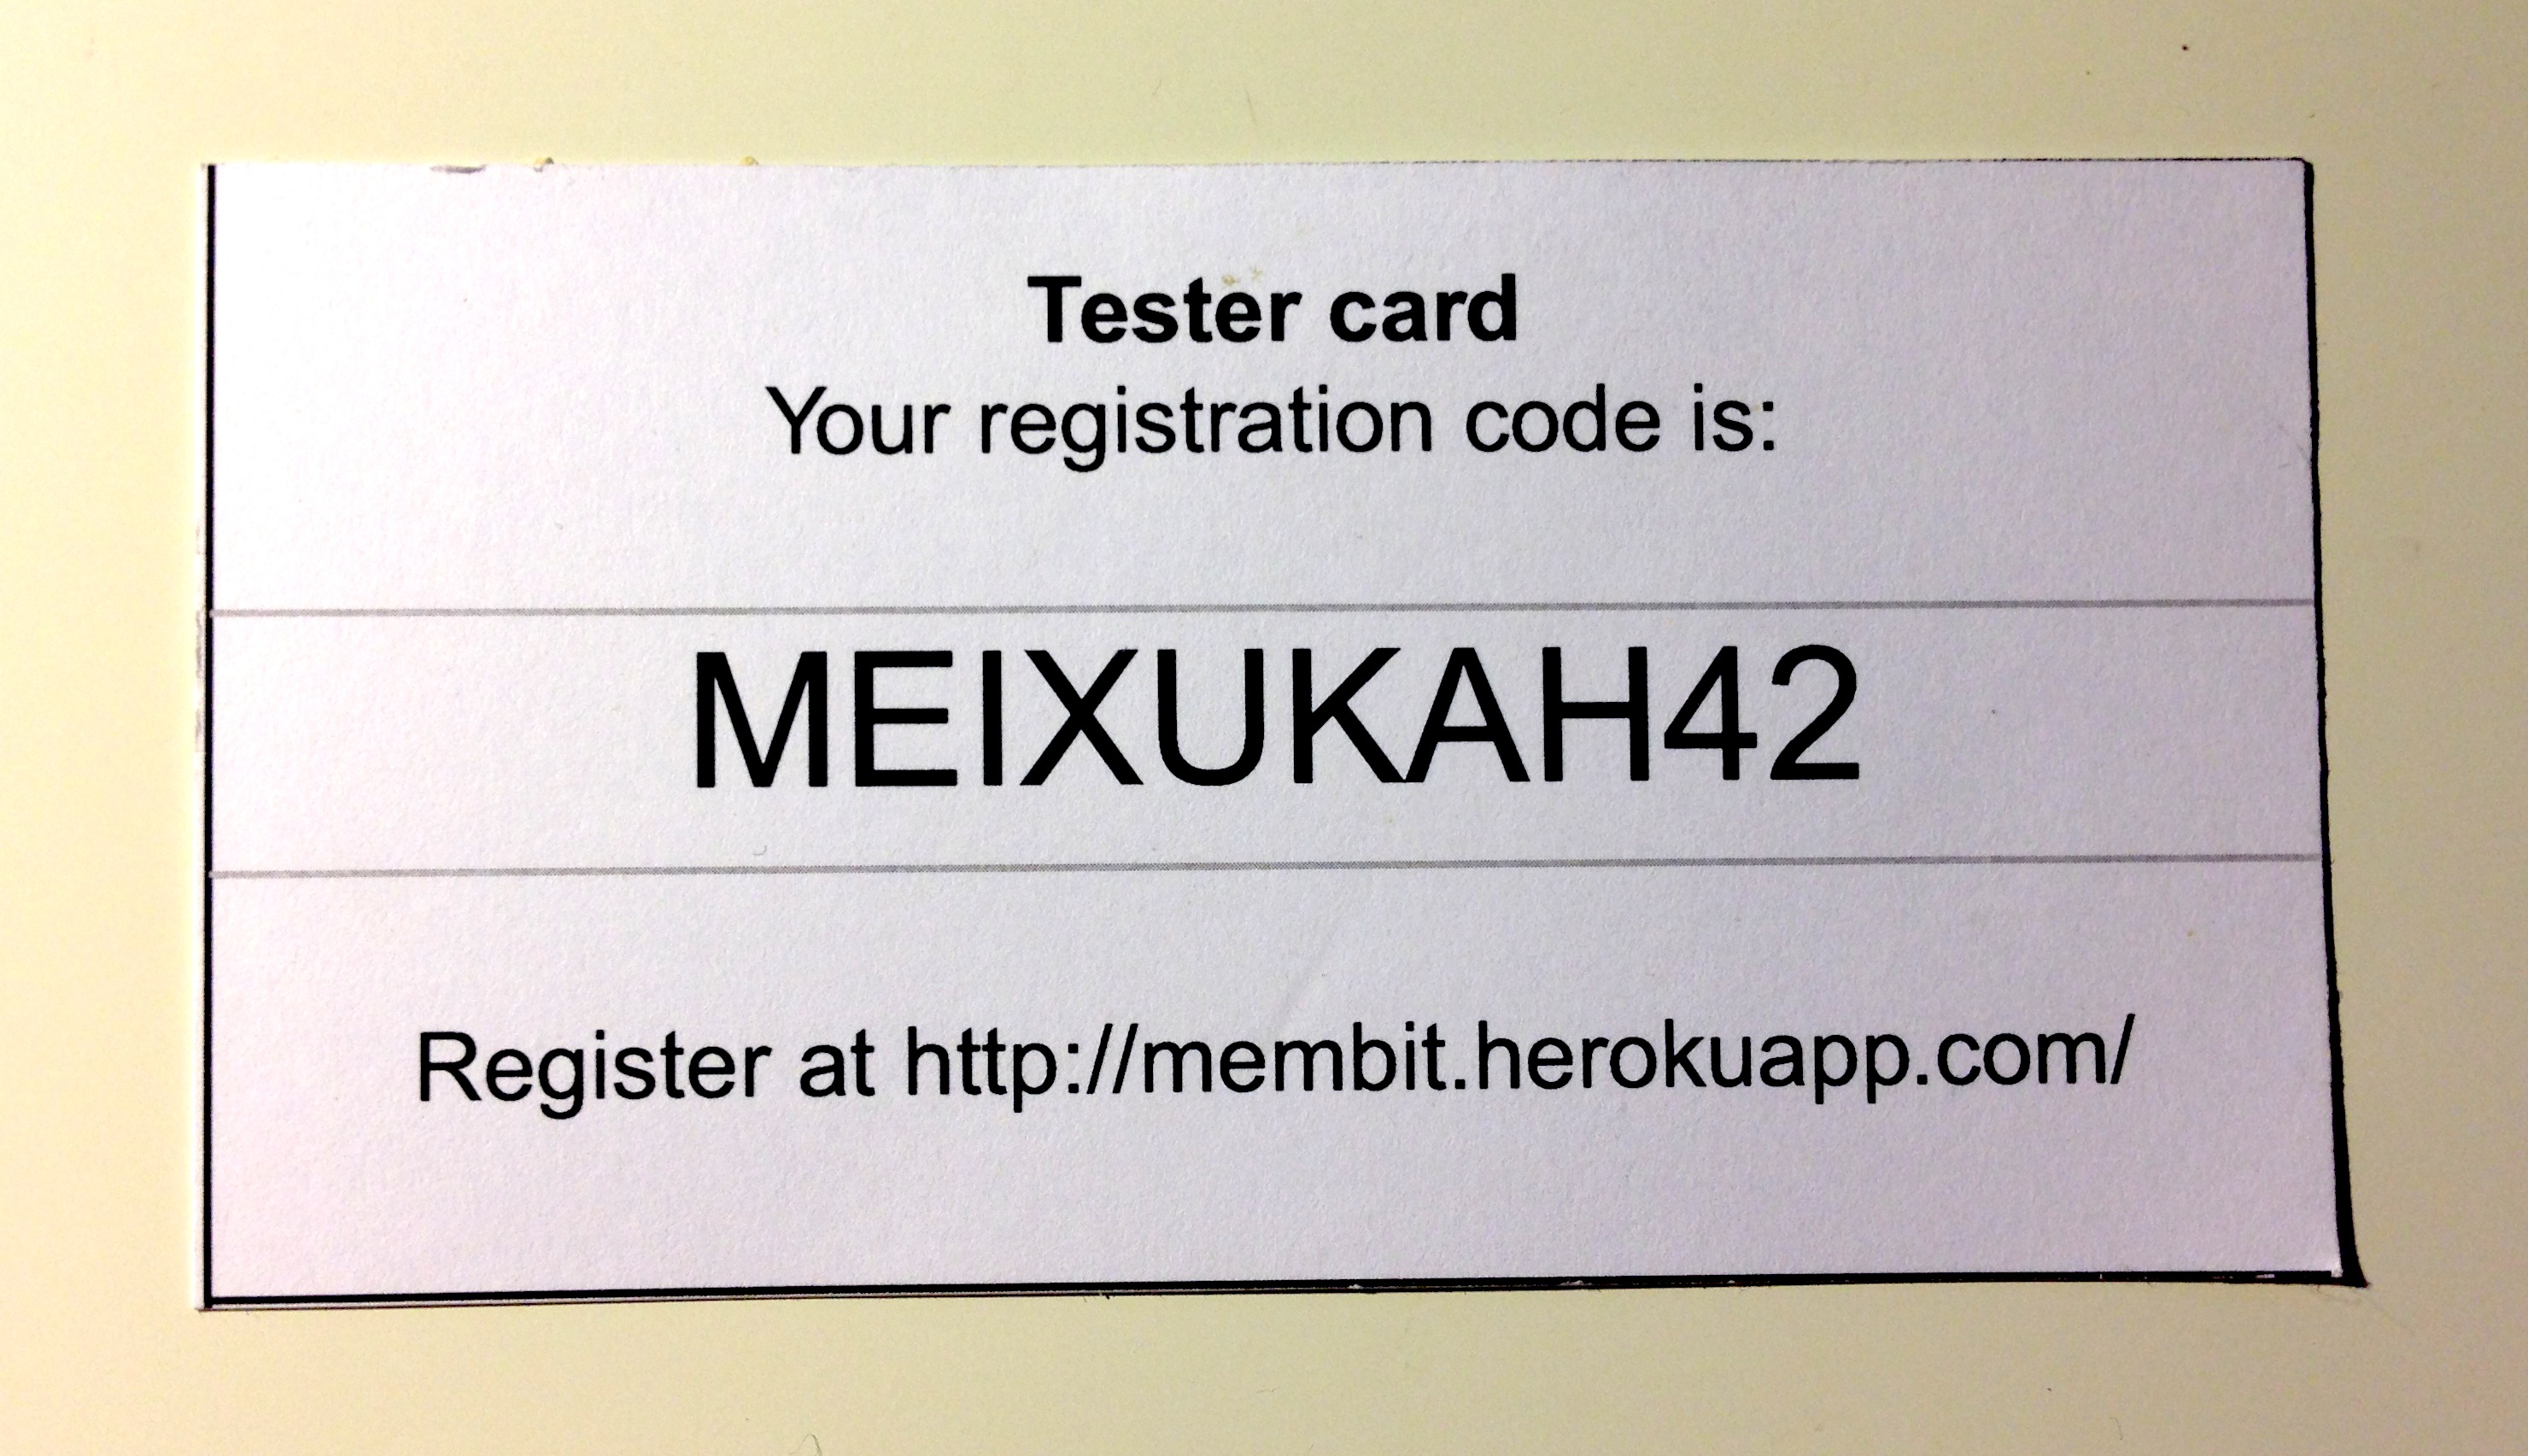
\includegraphics[width=9cm]{img/reg_card.jpeg}}
\caption{Sample registration card for a tester}
\label{fig_registrationcodes}
\end{figure}

\subsubsection{Teacher Dashboard}
A common feature in online learning environments is a dashboard for teachers to track
student usage. A basic dashboard was designed to visualise usage of the system
over time and to show information on the vocabulary list - which words were difficult
and which were not so difficult for students to remember.

\subsection{Vocabulary List}
The vocabulary selected was the vocabulary for the JAPN1023 course in which the participants
were enrolled. It is hoped that since the vocabulary is part of the course content, students
will be encouraged to use the software to learn the vocabulary. A total of 240 words were
entered into the database. 

The vocabulary was entered into a spreadsheet and run by the course coordinator for verification.
The vocabulary list was then exported to a .csv file and text manipulation software
was used to convert the list to Ruby code which inserts records directly into the
database. A .csv import mechanism was considered to replace this process, however
since the import is a one-time process this was decided against.  

\subsection{Spaced Repetition Algorithm Implementation}
The spaced repetition algorithm was implemented in Ruby as part of the application.
Data is stored in an SQL database. The variables required for the spaced repetition
algorithm are stored in a `UserWords' table which contains a record for each individual
user and vocabulary item. This means each time a new user is created, 240 records are added to the
`UserWords' table to keep track of each word. Upon review, the variables are pulled from this
table, recorded in
the reviews table along with the user's response 
and then a new interval and easiness factor calculated based on the previous
values and the user response.

In order to provide more review data at smaller intervals, the interval for the second 
repetition was halved from the original SuperMemo 2 algorithm from 6 days to 3 days.
This also affects subsequent reviews since each new interval is calculated on the
previous interval.

The same 0 to 5 rating system was used for the SuperMemo 2 algorithm, with a description of
each rating written beside the review interface. As with the original SuperMemo 2 algorithm,
if a user fails a review -- that is, selects 
a response from 0 to 2 -- the repetition number is reset to zero and thus the interval
reset. A flag is set against that item recording it as `failed' and it is shown
again to the user in the same session until they recall the item correctly.
The easiness factor however is not reset on failing an item and is calculated as per usual.

The system selects cards for the user to review in the following order:
\begin{enumerate}
  \item Cards due for review
  \item Failed cards
  \item New cards
\end{enumerate}

\subsection{Data storage, formatting and output}

The application data is stored in an SQL database accessed with the Ruby on Rails
framework. The following tables contain the major functionality:

\begin{description}
\item[Users] A listing of all registered users, and a secure one-way hash of their password information
to provide login functionality.
\item[Words] A listing of all 240 vocabulary items and their associated expression, meaning and readings.
\item[UserWords] Records spaced repetition parameters for a particular user and word association.
Each user has their own record of progress with each individual word.
\item[Reviews] Records of every review completed with the software. A review captures the current state
the associated UserWord record when a review is completed, and the user's selected answer for that review.
The review table keeps track of a user's role so that teacher, administrator and tester review data
can be removed when the data is exported leaving only participant review data.
\item[UserLogins] Records each `login' by each user. Since users are not automatically logged out,
a login is recorded whenever a student uses the software after a minimum 15 minute break.
\item[UserInfos] Contains demographic data on the users - their gender and whether English is their first language.
\end{description}

A full listing of tables and fields is available in the /db/schema.rb file in the Membit source code.


Review data is made available via an administrator login. The software converts the
table of anonymised participant reviews to a .CSV file for download. CSV was chosen because of its portability --
almost all data analysis packages support CSV files. Data could also be filtered before download, 
to remove unwanted entries. Most importantly, it was made possible to filter out `new' reviews, ie.
reviews for which it was the first time for a student to study a word. These reviews contain almost
no useful data for prediction since there is no history for that student reviewing that word.

Fields contained in the downloaded review data are described in table \ref{tbl_csvfields}

\begin{table}
\caption{Fields contained within downloaded data files}
\label{tbl_csvfields}
\begin{tabular}{|p{4cm}|c|p{9cm}|}
\hline
Field & Type & Description \\
\hline
User Word ID  & ID & A unique ID for a user and vocabulary item pair (a user-word). \\
Word ID  & ID & A unique ID for each vocabulary item. \\
User ID  & ID & A unique ID for each user. \\
Was New? & Boolean & True if this is the first time the user has studied this vocabulary item. False otherwise. \\
Overdue Time & Continuous & Number of days after the vocabulary item was due for review that it was studied.\\
Previous Incorrect Count & Discrete & Number of times this vocabulary item \textbf{has not} been recalled correctly before this review. \\
Previous Correct Count & Discrete & Number of times this vocabulary item \textbf{has} been recalled correctly before this review. \\
Previous Easiness Factor & Continuous & The easiness factor that was assigned to this vocabulary item for this user before this review. \\
User Rated Answer & Discrete & The answer the student selected (0 - 5) \\
Time to Answer & Continuous & The amount of time between seeing the front of the flash-card and selecting an answer. \\
Correct? & Boolean & Whether the recall was considered correct. FALSE if answer selected was 0-2, TRUE if 3-5. \\
Previous Repetition Number & Discrete & The repetition number before this review. NULL = This is the first review, 0 = The previous review was the first. Note that this number is reset after a card is failed. \\
Previous Interval  & Continuous & The interval, or amount of time between the previous review and the due date for this review. \\
Actual Interval & Continuous & The actual time between the previous review and the current review.\\
Was Failed? & Boolean & Whether the user-word was failed on the previous review. TRUE if the card was failed before this review, FALSE if the card was not failed.\\
Previous Attempts & Discrete & Total number of attempts at reviewing this user-word prior to this review \\
Previous Answer & Discrete & The user rated answer of the previous review \\
Previous Time to Answer & Continuous & The time the user took to answer on the previous review\\
Word Average Easiness Factor & Continuous & Average easiness factor for this word for all users\\
\hline
\end{tabular}
% Use own page
\vspace*{4cm}
\end{table}

\section{Data Analysis and Prediction}
\subsection{Forgetting Curves}

Forgetting curves can be generated from the recorded reviews by grouping review data on the following
variables:
\begin{itemize}
  \item Repetition number
  \item Actual interval
\end{itemize}

Given these groups, the chance of remembering a fact for a specific repetition number and interval 
can be estimated with equation \ref{eqn_forgettingcurveprob}:

\begin{equation}
\label{eqn_forgettingcurveprob}
P(correct,incorrect) = \frac{\sum correct}{\sum correct + \sum incorrect}
\end{equation}

However with groups of data for which there is minimal review data, this equation will yield
large errors. For example, if a grouping of data is as shown in table \ref{tbl_forgettingcurvegrouping}:

\begin{table}[h!]
\caption{Example of too few review samples after grouping}
\label{tbl_forgettingcurvegrouping}
\begin{tabular}{|c|c||c|}
\hline
Repetition Number & Actual Interval & Correct?\\
\hline
3 & 18 & TRUE\\
3 & 18 & FALSE\\
3 & 18 & FALSE\\
\hline
\end{tabular}
\end{table}

Given the sample of the three reviews in table \ref{tbl_forgettingcurvegrouping}
-- equation \ref{eqn_forgettingcurveprob} would yield $P = \frac{1}{1+2} = 0.333$.
However the standard error as calculated with equation \ref{eqn_standarderror} yields
$\sqrt{\frac{0.333(1 - 0.333)}{3}} = 0.272$

\begin{equation}
\label{eqn_standarderror}
\text{Standard Error} = \sqrt{\frac{p(1-p)}{n}}
\end{equation}

We cannot say with any accuracy from this data that the probability of remembering a word
given these inputs is 0.333. On the other hand, with a sampling of thousands of reviews for a
given repetition number and actual interval the error is reduced and a probability can
be considered more accurate. %TODO Probability Ref

This issue is one of gathering enough data, and so various thresholds for minimum number of reviews
to give an adequate probability will be arbitrarily selected based on the amount of data available.

Forgetting curves can also be generated from running data through the machine learning
algorithms trained upon the data. By entering a full range of possible variable values through
the trained machine learning algorithms, we can generate a much larger dataset than original
to work with. This will also be explored and compared with the forgetting curves generated from
the true data.

Due to the limited amount of data expected, forgetting curves will be constructed on the basis of
the entire set of users and not for individual users.

\subsection{Prediction of Recall}

Prediction of recall is carried out using the R programming language and packages
which implement machine learning algorithms. Packages used include:
\begin{description}
\item[e1071] An implementation of libsvm, a common Support Vector Machine library
\item[nnet] A neural network implementation supports multilayer perceptrons with 
logistic and linear outputs.
\end{description}

The review data is downloaded as .csv from the administration section of the online
learning environment. An R script loads the .csv file into the environment, strips
out the irrelevant columns in the data, trains and validates the selected 
machine learning algorithms on the data. Table \ref{tbl_inputoutputs} shows
the variables that are kept from the review data and their usage for training
and validation. Note that the output `Correct' is calculated based on the `User
Rated Answer' and is simply a convenience to refer to whether or
not the user correctly recalled a word without taking into account the subjective
difficulty of recall.

The inputs shown in table \ref{tbl_inputoutputs} are the same variables which are
either stored or can be calculated from values stored alongside each user-word in
the database by the spaced repetition algorithm. This means that given a well
trained algorithm and a set of user-words for a user, it should be possible to
calculate which words the user will correctly recall at any given point in time.

\begin{table}[h!]
\caption{Inputs and Outputs to Machine Learning Algorithms}
\label{tbl_inputoutputs}
\begin{tabular}{|c|c|c|}
\hline
Field & Type & Input/Output \\
\hline
Overdue Time & Continuous & Input \\
Previous Incorrect Count & Discrete & Input \\
Previous Correct Count & Discrete & Input \\
Previous Easiness Factor & Continuous & Input \\
Previous Repetition Number & Discrete & Input \\
Previous Interval & Continuous & Input \\
Actual Interval & Continuous & Input \\
Previous Attempts & Discrete & Input \\
Previous Answer & Discrete & Input \\
Previous Time to Answer & Continuous & Input \\
Word Average Easiness Factor & Continuous & Input \\
\hline
User Rated Answer & Discrete & Output \\
Correct & Boolean & Output \\
\hline
\end{tabular}
\end{table}